\documentclass[10pt]{beamer}    
\usetheme{Dresden}
%\usepackage[margin=2cm]{geometry} 

\usepackage{amsmath}   
\usepackage{amsfonts}
\usepackage{physics}     
\usepackage{siunitx} 
\usepackage{graphicx}
\usepackage{subfigure}
%\usepackage{caption}
\usepackage{verbatim}
\usepackage{float}
%\usepackage{svg}
\usepackage{vwcol}

\setlength\parindent{0pt}
\setlength\parskip{5pt}


\newcommand\numberthis{\addtocounter{equation}{1}\tag{\theequation}}
\DeclareMathOperator{\lagr}{\mathcal{L}}
\DeclareMathOperator{\ham}{\mathcal{H}}

\title{Numerical Characterisation of the Trifluxonium Superconducting Qubit}
\subtitle{Advisor: Andrew Houck}
\author{Shiye Su}
\institute{Princeton University}
%\date{\today}
\date{}

\begin{document}



\begin{frame}
\titlepage
\end{frame}


\begin{frame}
\frametitle{Quantum bits}
\begin{itemize}
\item superposition property $\rightarrow$ speedups (Shor 1994, Grover 1995)
\item qubits: two state system
\item superconducting circuit: discrete energies at microwave spacing, control and readout via cavity QED.
\end{itemize}
\end{frame}

% architecture upon robust and long-lived qubits. initialisable, long coherence times relative to gate speed
% a solid state implementation. industry dominant.
% physical picture: etched plate in a cavity in dilution refrigerator. minimise flux


\begin{frame}[shrink=10]
\frametitle{Dynamic variables}
\vspace{3ex}
branch fluxes $\phi(t)$ (`position') and branch charges $q(t)$ (`momenta')
\begin{equation}
\phi(t) = \int_{-\infty}^t V(\tilde{t}) \dd{\tilde{t}}
\hspace{2cm}
q(t) = \int_{-\infty}^t I(\tilde{t}) \dd{\tilde{t}}
\end{equation}

\begin{equation}
\varphi(t) \equiv \frac{\phi(t)}{\phi_0}
\quad \phi_0 \equiv \frac{\hbar}{2e}
\hspace{2cm}
n(t) = \frac{1}{2e} q(t)
\end{equation}

dispersive elements
\begin{equation}
E_\text{capacitor} = \frac{1}{2} C \dot{\phi}^2, 
\quad
C(q) \equiv \left( \dv{v(q(t))}{q} \right)^{-1}
\end{equation}
\begin{equation}
E_\text{inductor} = \frac{1}{2L} \phi^2,
\quad
L(\phi) \equiv \left( \dv{I(\phi(t))}{\phi} \right)^{-1}
\end{equation}
\end{frame}

% generalised coordinates in Lagrangian and Hamiltonian formulation
% ideal linear elements. purely capacitative - voltage pure function of charge, purely inductive - current pure function of flux
% conservative elements (not resistor). ideal linear
% we will use Hamiltonian, eigensystem characterises. corresponding Euler-Lagrange and Hamilton's equations if we're interested in dynamics


\begin{comment}
cooper pairs, condensate in ground state
\begin{equation}
\psi(\vec{r}) = \sqrt{\rho(\vec{r})} e^{i \theta(\vec{r})}
\end{equation}
supercurrent density
\begin{equation}
J(\vec{r},t) = \frac{\hbar}{m} \left(\nabla \theta - \frac{q}{\hbar} \vec{A} \right) \rho
\end{equation}
\end{comment}

\begin{frame}
\frametitle{Josephson junction}
\vspace{3ex}

\begin{equation}
I(t) = \frac{\phi_0}{L_J} \sin{\varphi_J(t)}
\end{equation}
\begin{equation}
E(t) = -\frac{\phi_0^2}{L_J} \cos{\varphi(t)}
\end{equation}

\begin{figure}[H]
	\centering
	\subfigure{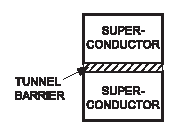
\includegraphics[width=0.25\textwidth]{jj_schematic.pdf}}
	\subfigure{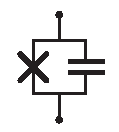
\includegraphics[width=0.18\textwidth]{jj_circuit.pdf}}
	\subfigure{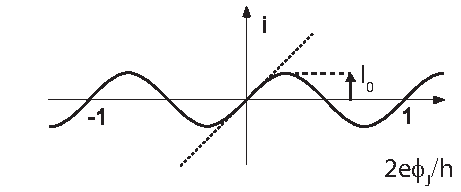
\includegraphics[width=0.5\textwidth]{jj_current.pdf}}
	\caption{Physical schematic, circuit, current-flux relation.}
\end{figure}
\end{frame}

% derivation: weakly connected superconductors, supercurrent density in a bulk supercurrent depends on gauge invariant phase gradient. apply the probability density oeprator, get basically the difference between the phases, enforce 2\pi periodidc, drop higher harmonics
% probability current \frac{1}{2m} (\psi^* p \psi - \psi p \psi^*)


%$ \phi \rightarrow \hat{\phi}, \quad
%q \rightarrow \hat{q}, \quad
%\ham \rightarrow \hat{\ham}
%$

%\begin{equation}
%q = \pdv{\lagr}{\dot{\phi}}
%\hspace{1cm}
%q = -i \hbar \pdv{}{\phi}
%\hspace{1cm}
%\comm{\hat{\phi}}{\hat{q}} = i \hbar
%\end{equation}

\begin{frame}[shrink=10]
\frametitle{Quantisation and setup}
\vspace{3ex}

$\varphi$, $n$ are operators
$\varphi$, $n$ are conjugate variables

\begin{equation}
n = \frac{1}{\hbar} \pdv{\lagr}{\dot{\varphi}}
\hspace{1cm}
n = -i\pdv{}{\varphi}
\hspace{1cm}
\comm{\hat{\varphi}}{\hat{n}} = i
\end{equation}

Writing the Lagrangian:
\begin{equation}
E_\text{capacitor} = \frac{1}{2} C \phi_0^2 \dot{\varphi}^2
\hspace{1cm}
E_\text{inductor} = \frac{1}{2} E_L \varphi^2
\hspace{1cm}
E_\text{junction} = - E_J \cos{\varphi}
\end{equation}

system description
\begin{equation}
\lagr\left(\{\phi\}, \{\dot{\phi}\}\right) = T(\dot{\phi}) - V(\phi),
\quad
\ham = \pdv{\lagr}{\dot{\phi}_i} \dot{\phi}_i - \lagr
\end{equation}

%With constraint: 
%$ \sum_\text{around loop} \phi = \phi_\text{ext} $.

\end{frame}

% analogy to x and p
% Note: we choose to use (continuous) phase basis.


\begin{frame}[shrink=20]
\frametitle{Cooper pair box}

\begin{figure}
	\centering
	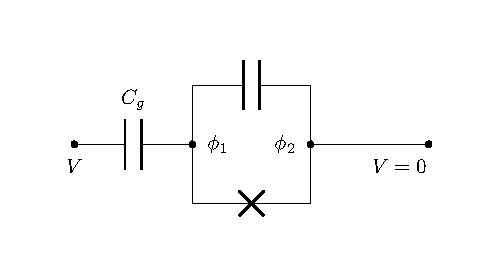
\includegraphics[trim={0cm 1cm 0cm 1cm}, clip, width=0.5\textwidth]{cpb.pdf}
\end{figure}
capacitatively coupled CPB.

\begin{equation}
\lagr 
= \frac{1}{2} C_g (\dot{\phi}_1 - V)^2 + \frac{1}{2} C (\dot{\phi}_1 - \dot{\phi}_2)^2 + E_J \cos{\left(\frac{\phi_1 - \phi_2}{\phi_0}\right)} 
\end{equation}

\begin{equation}
\theta = \frac{1}{2} (\varphi_1 - \varphi_2)
\hspace{1cm}
\Sigma = \frac{1}{2} (\varphi_1 + \varphi_2)
\end{equation}

\begin{equation}
\boxed{ \ham = 4 E_C (- i \partial_\theta - n_g)^2 - E_J \cos{\theta} }
\end{equation}

\end{frame}

% E_C = \frac{e^2}{2 (C + C_g)}, \quad n_g = - \frac{C_g V}{2e}

% capacitance is lumped from capacitor and cooper pair box
% key idea: compact variable. drop it in final expression. 
% notice the anharmonic cosine potential

\begin{frame}
\frametitle{Energy spectrum and the transmon regime}

\begin{figure}
	\centering
	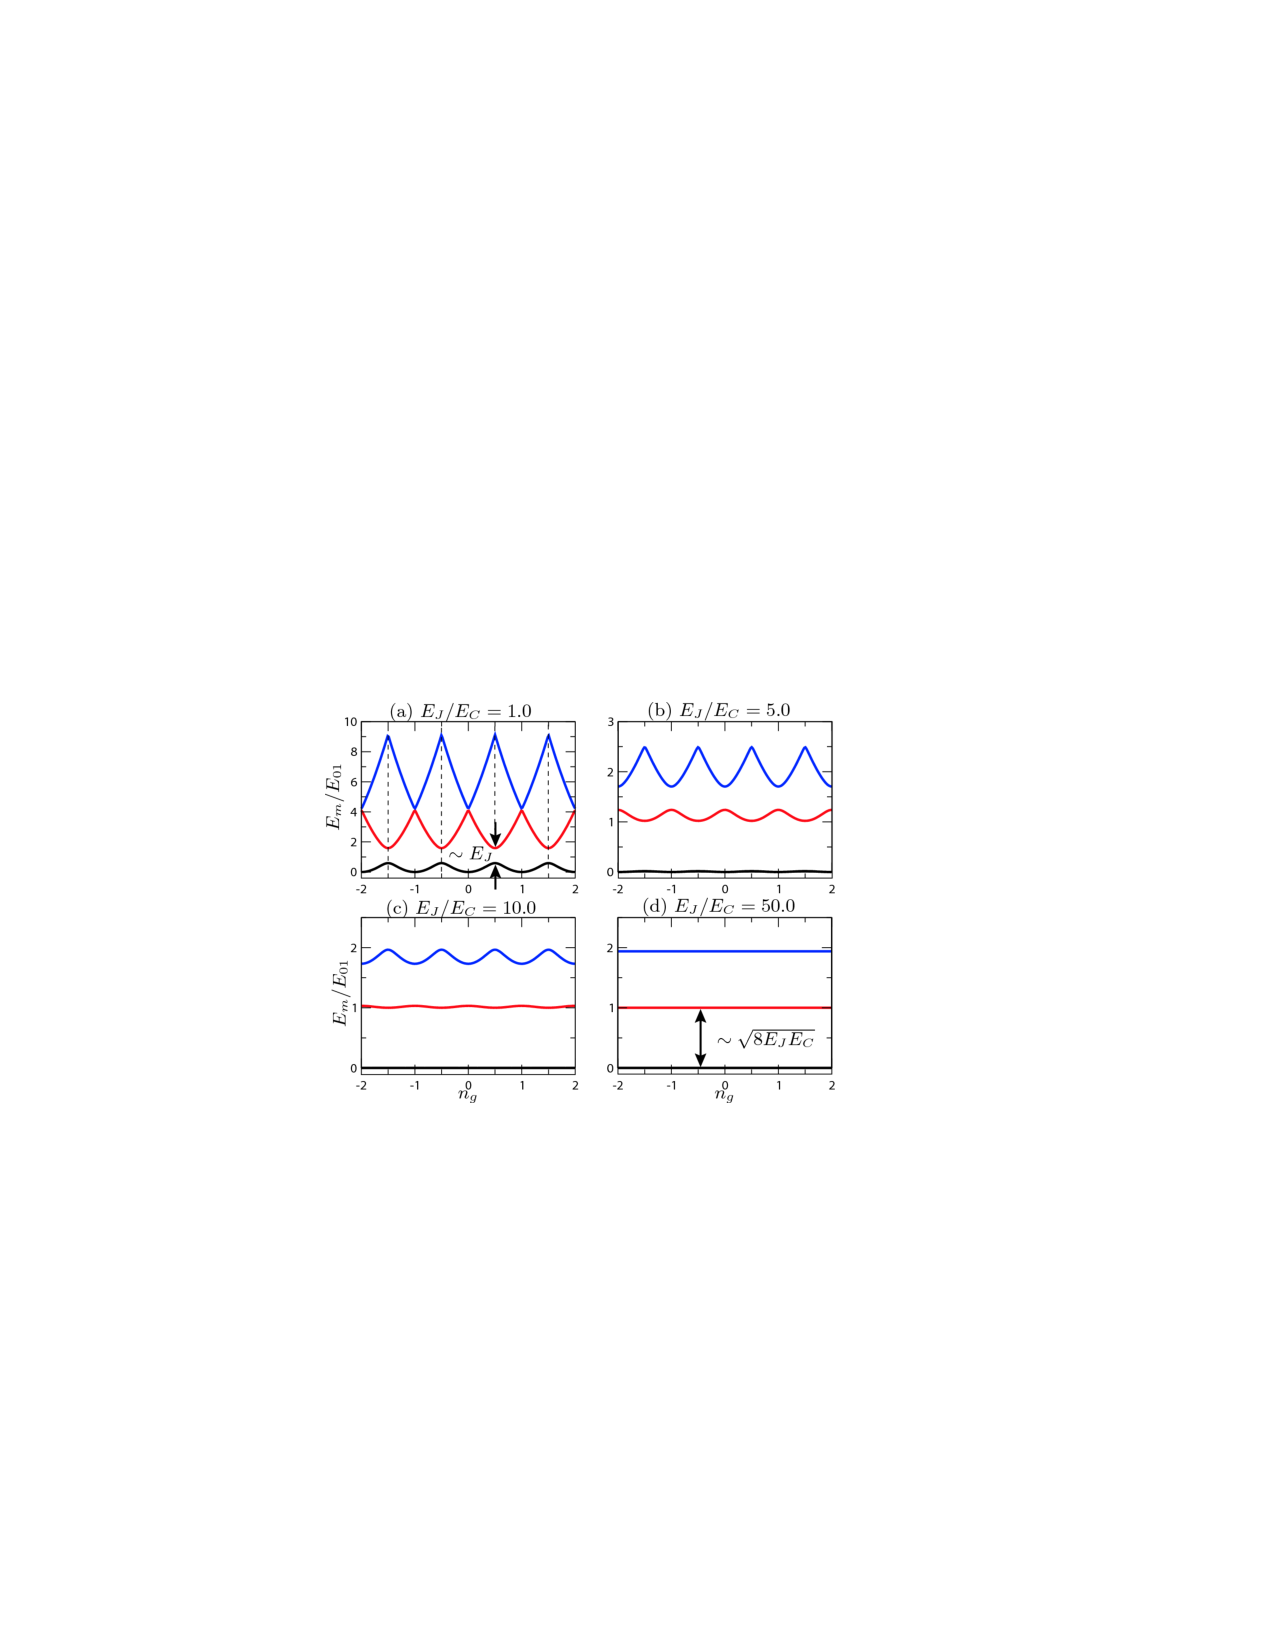
\includegraphics[width=0.6\textwidth]{cpb_energies.pdf}
\end{figure}

\begin{itemize}
\item $n_g$ dependence
\item \emph{transmon}: $\ket{0}-\ket{1}$ transition frequency preserved
\item limitations: approaches harmonic LC-oscillator, not disjoint
\end{itemize}

\end{frame}

% First three CPB eigenenergies as a function of $n_g$. Energies in units of transition energy $E_{01}$ evaluated at $n_g=1/2$.
% typically we choose ground state t0 be 0, first excited to be 1
% localisation, susceptible to ground state relaxation, $T_1$



\begin{frame}
\frametitle{Fluxonium}
\vspace{1ex}
\begin{minipage}[c]{0.4\linewidth}
\begin{figure}
	\centering
	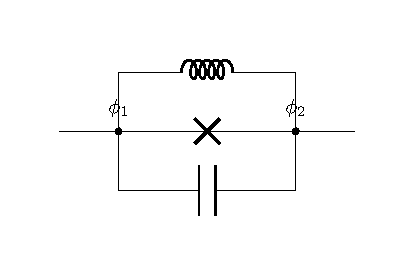
\includegraphics[trim={1cm 1cm 1cm 1cm}, clip, width=0.7\textwidth]{fluxonium.pdf}
\end{figure}
\end{minipage} 
\begin{minipage}[c]{0.5\linewidth}
\begin{equation}
\footnotesize
\boxed{ \ham = - 4 E_C \partial_\varphi^2  - E_J \cos{\left(\varphi - \frac{\phi_E}{\phi_0}\right)} + \frac{1}{2} E_L \varphi^2 }
\end{equation}
\end{minipage}
\begin{figure}[H]
	\centering
	\subfigure[$\varphi=0.02(2\pi)$.]{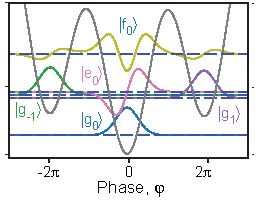
\includegraphics[width=0.35\textwidth]{fluxoniumenergies1.pdf}}
	\subfigure[$\varphi=0.51(2\pi)$.]{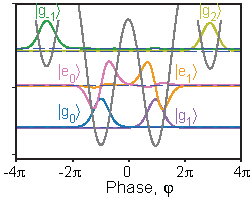
\includegraphics[width=0.34\textwidth]{fluxoniumenergies2.pdf}}
\end{figure}
\begin{itemize}
\item Disjoint $\matrixel{0}{n}{1} \approx 0$. Transition via excited level.
\item Sensitivity to external flux. Dephasing. Relaxation. 
\end{itemize}
\end{frame}

% the same change of variables diagonalises the potential

% Potential landscape and eigensystem for two $\phi_\text{ext}$. Notice (b) quasi symmetric double well with near degenerate $\ket{g_0}$ and $\ket{g_1}$.



\begin{frame}[shrink=20]

\frametitle{Trifluxonium}

\vspace{0.5cm} 

\begin{columns}
\column{0.5\textwidth}
\begin{figure}
	\centering
	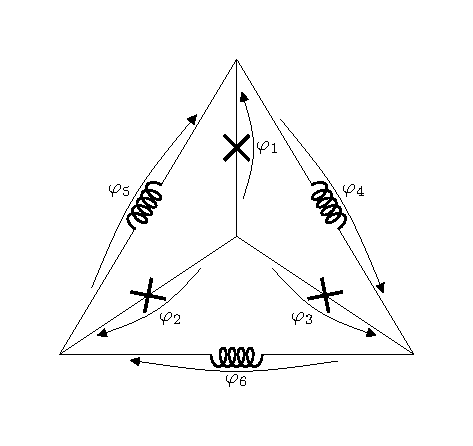
\includegraphics[trim={0cm 1cm 0cm 1cm}, clip, width=0.9\textwidth]{triflux_branch.pdf}
\end{figure}
\column{0.5\textwidth}
Parameters: $E_L$, $E_J$, $E_C$.
Dyanamic variables: $\zeta, \theta, \chi$.
\end{columns}

\vspace{0.5cm}

\begin{align*}
\ham = -4 E_C & \left( \partial_\zeta^2 + \partial_\theta^2 + \partial_\chi^2 \right) - \\
& E_J \left( \cos{\left(\frac{\zeta + \sqrt{2} \chi}{\sqrt{3}}\right)} + 2 \cos{\left(\frac{\theta}{\sqrt{2}}\right)} \cos{\left(\frac{\zeta}{\sqrt{3}} - \frac{\chi}{\sqrt{6}}\right)} \right) + \frac{3}{2} E_L (\theta^2 + \chi^2 + \varphi_E)
\end{align*}

Potential landscape?

$\varphi_E$ independent!


\end{frame}

% choose variables such that diagonalises the potential. again, a variable drops out



\setcounter{subfigure}{0}

\begin{frame}[shrink=10]
\frametitle{Eigensystem}

\begin{minipage}[c]{0.49\linewidth}

\vspace{2ex}

\small

Parameters:

$E_C = \SI{2}{\giga\hertz}$, $E_J = \SI{15}{\giga\hertz}$, $E_L = \SI{0.3}{\giga\hertz}$

\vspace{2ex}

Criteria:
\begin{itemize}
\item nondegeneracy
\item anharmonicity
\item insensitivity to external parameters
\item disjoint support with viable transition
\end{itemize}

\begin{table}[H]
	\footnotesize
	\centering
	\begin{tabular}{l l l}
		\hline
		Ground 		& Fluxons 			& Plasmons \\
		\hline
		$E_0 = 0$ 	& $E_1 = 10.88$		& $E_7 = 13.164$ \\
					& $E_2 = 10.881$ 	& $E_8 = 13.618$ \\
					& $E_3 = 10.9$		& $E_9 = 13.619$ \\
					& $E_4 = 10.954$ 	& \\
					& $E_5 = 10.954$ 	& \\
					& $E_6 = 10.97$		& \\
		\hline
	\end{tabular}
\end{table}
\end{minipage}
\begin{minipage}[c]{0.49\linewidth}
\begin{figure}
	\centering
	\subfigure{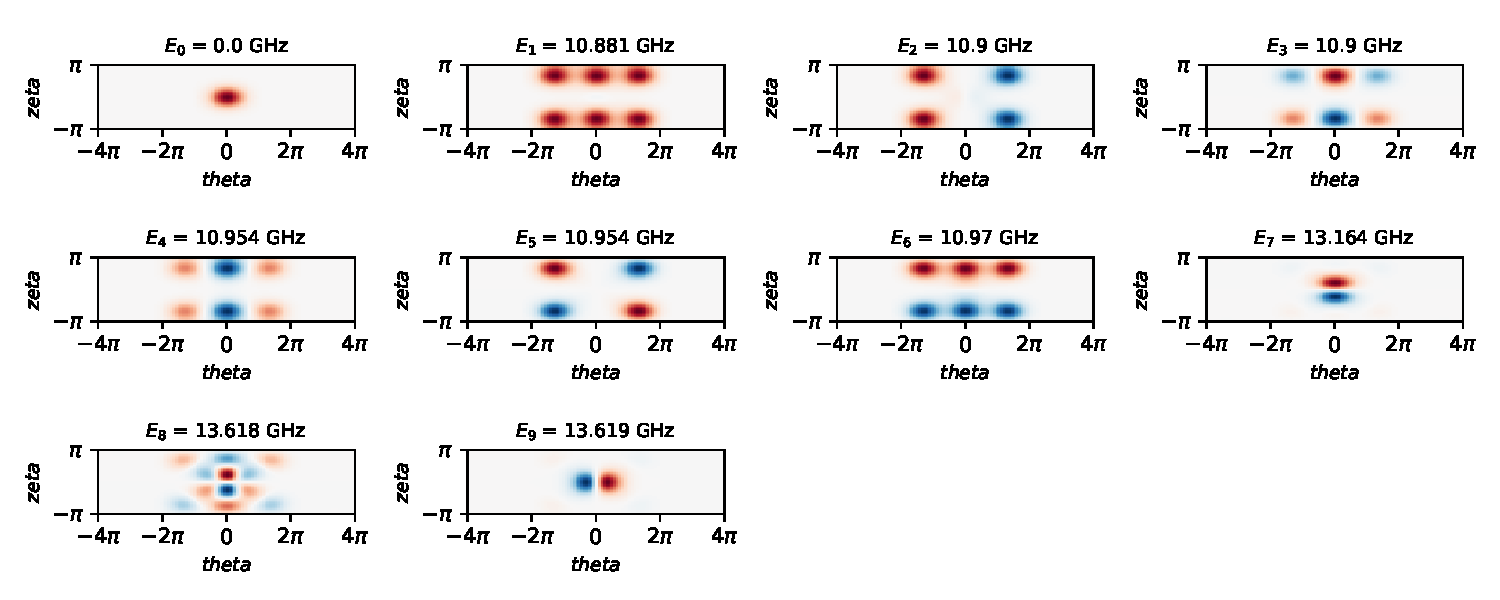
\includegraphics[trim={0cm 0.3cm 0cm 0cm}, clip, width=1\textwidth]{zetatheta.pdf}}
	\subfigure{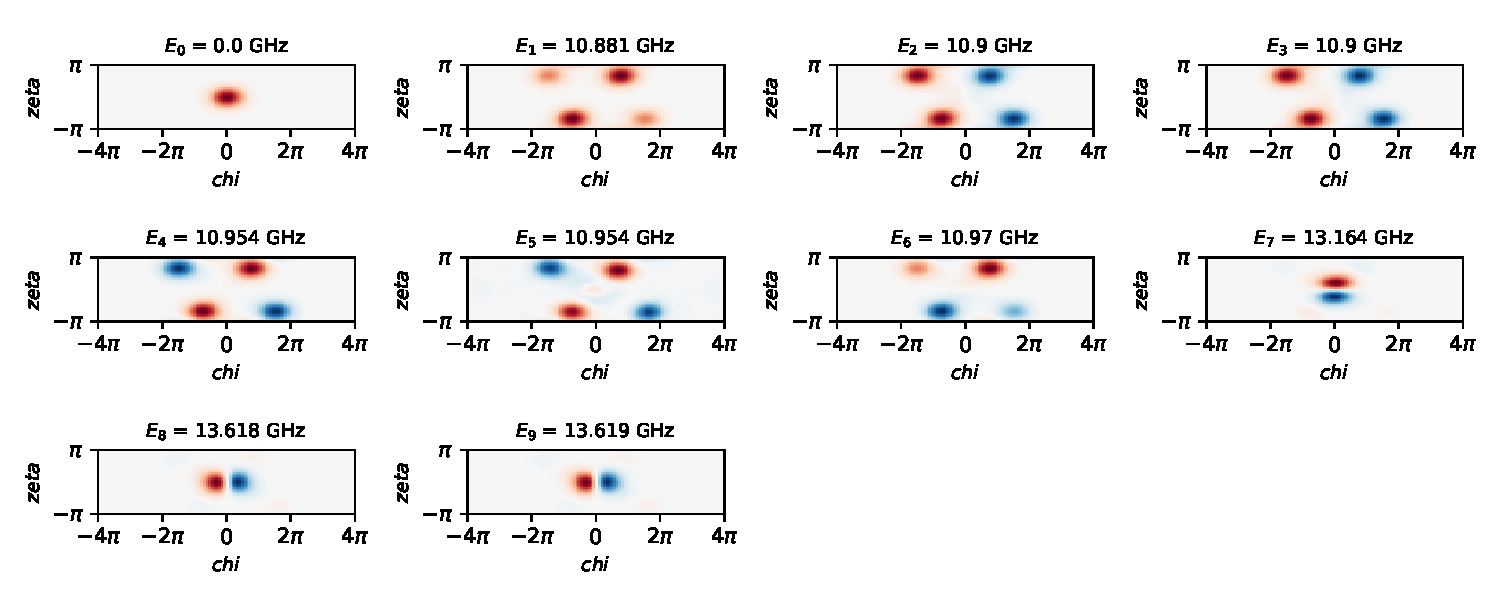
\includegraphics[trim={0cm 0.3cm 0cm 0cm}, clip, width=1\textwidth]{zetachi.pdf}}
	\subfigure{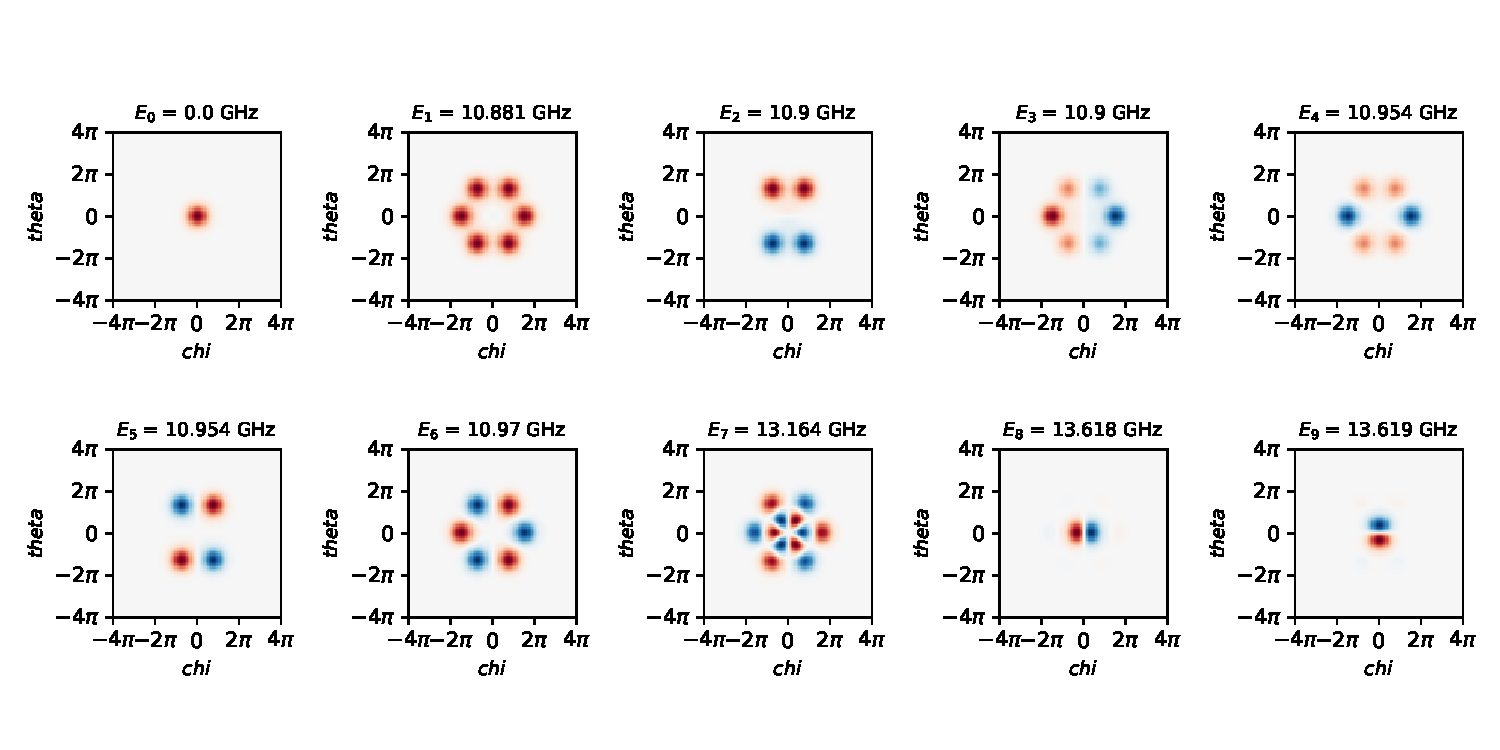
\includegraphics[trim={0cm 1.5cm 0cm 1cm}, clip, width=1\textwidth]{thetachi.pdf}}
\end{figure}
\end{minipage} 

\end{frame}

% three way symmetry results in degeneracies
% disjoint


\setcounter{subfigure}{0}

\begin{frame}[shrink=10]
\frametitle{Eigensystem}
\begin{figure}
	\centering
	\subfigure[$\ket{0}$, $\ket{1}$.]{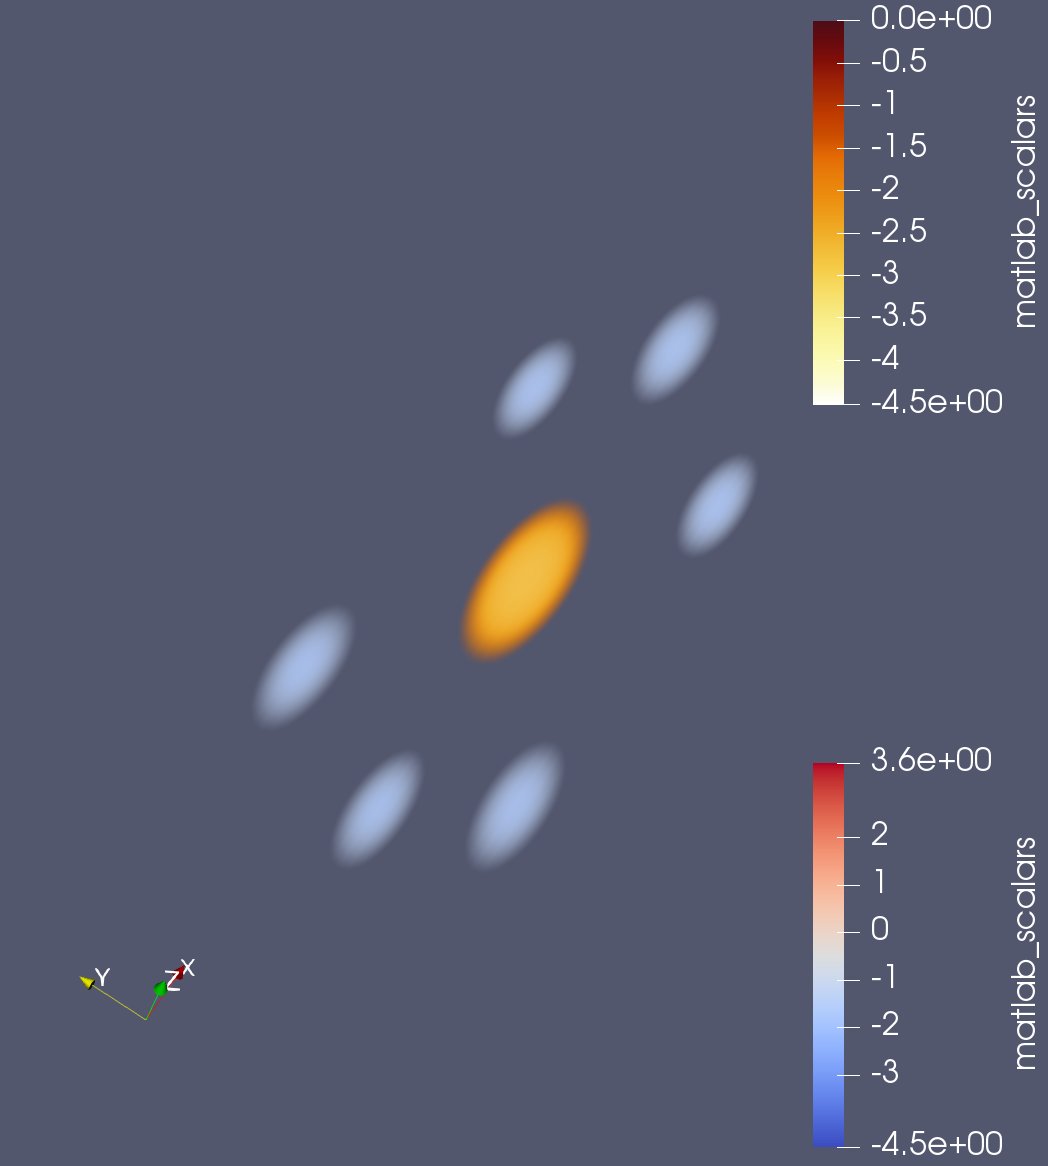
\includegraphics[width=0.25\textwidth]{ekets01.png}}
	\hspace{1em}
	\subfigure[$\ket{0}$, $\ket{2}$.]{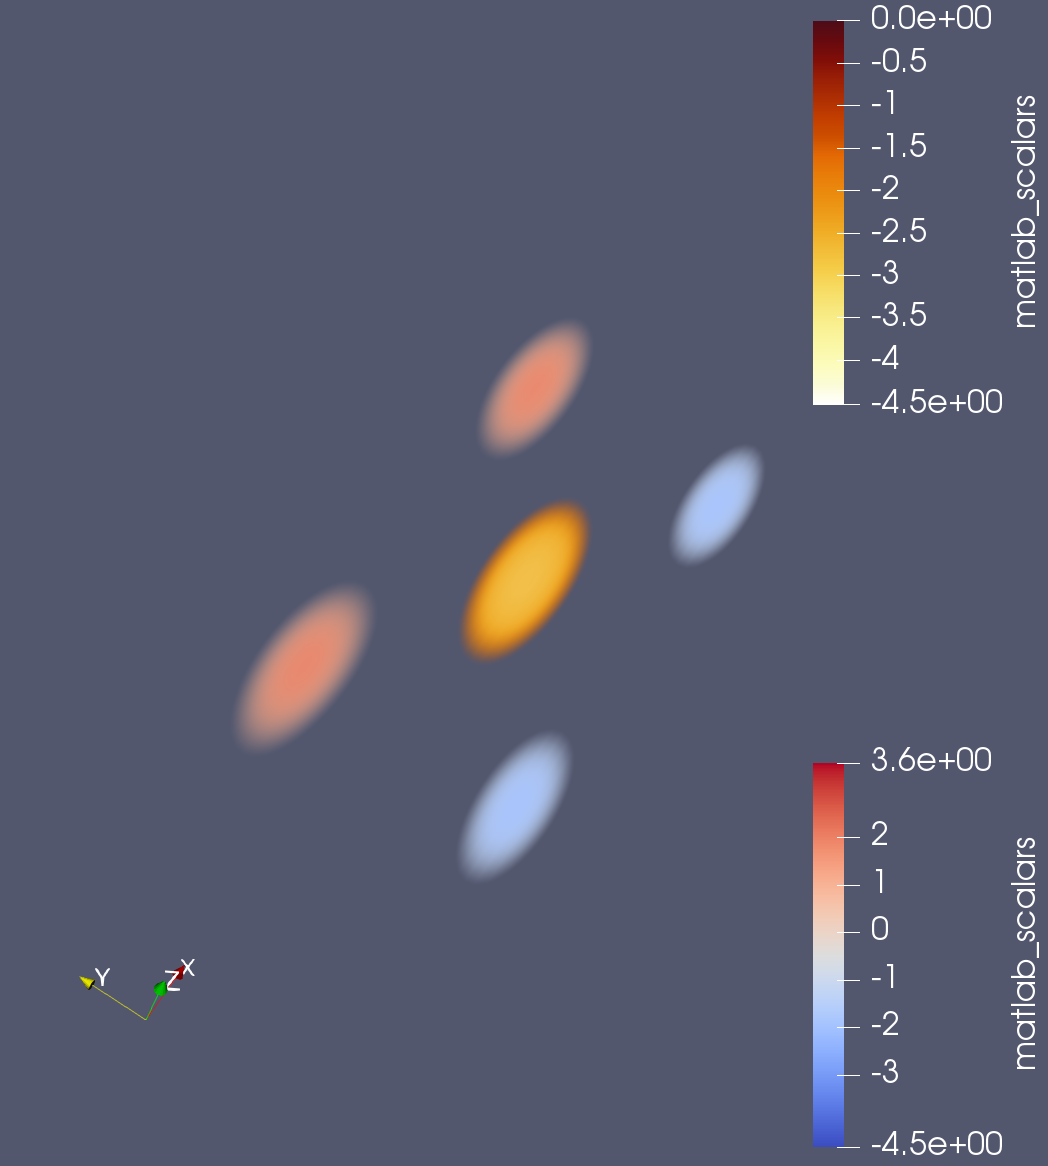
\includegraphics[width=0.25\textwidth]{ekets02.png}}
	\hspace{1em}
	\subfigure[$\ket{0}$, $\ket{3}$.]{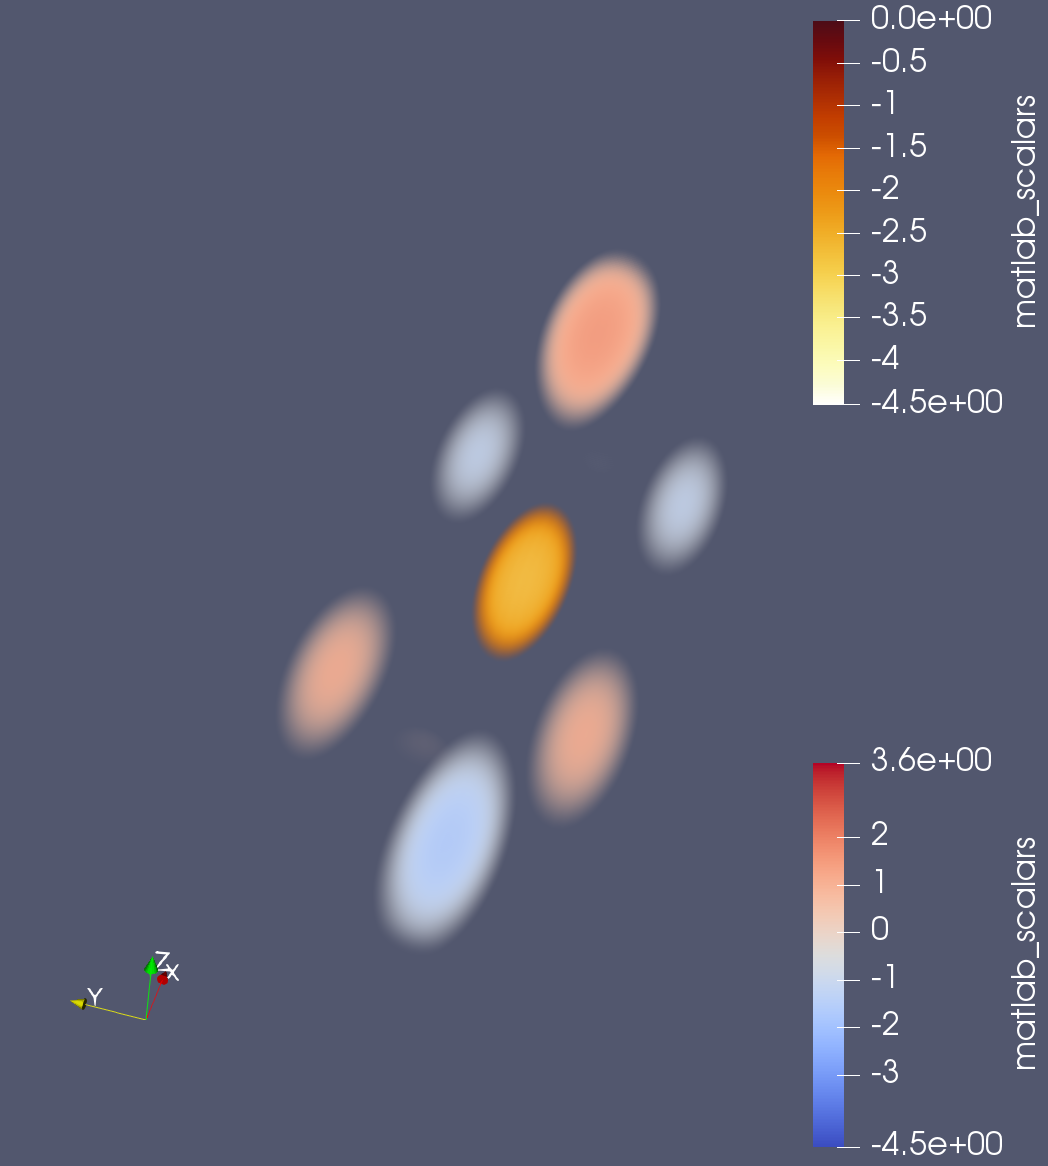
\includegraphics[width=0.25\textwidth]{ekets03.png}}
	\hspace{1em}
	\subfigure[$\ket{0}$, $\ket{7}$.]{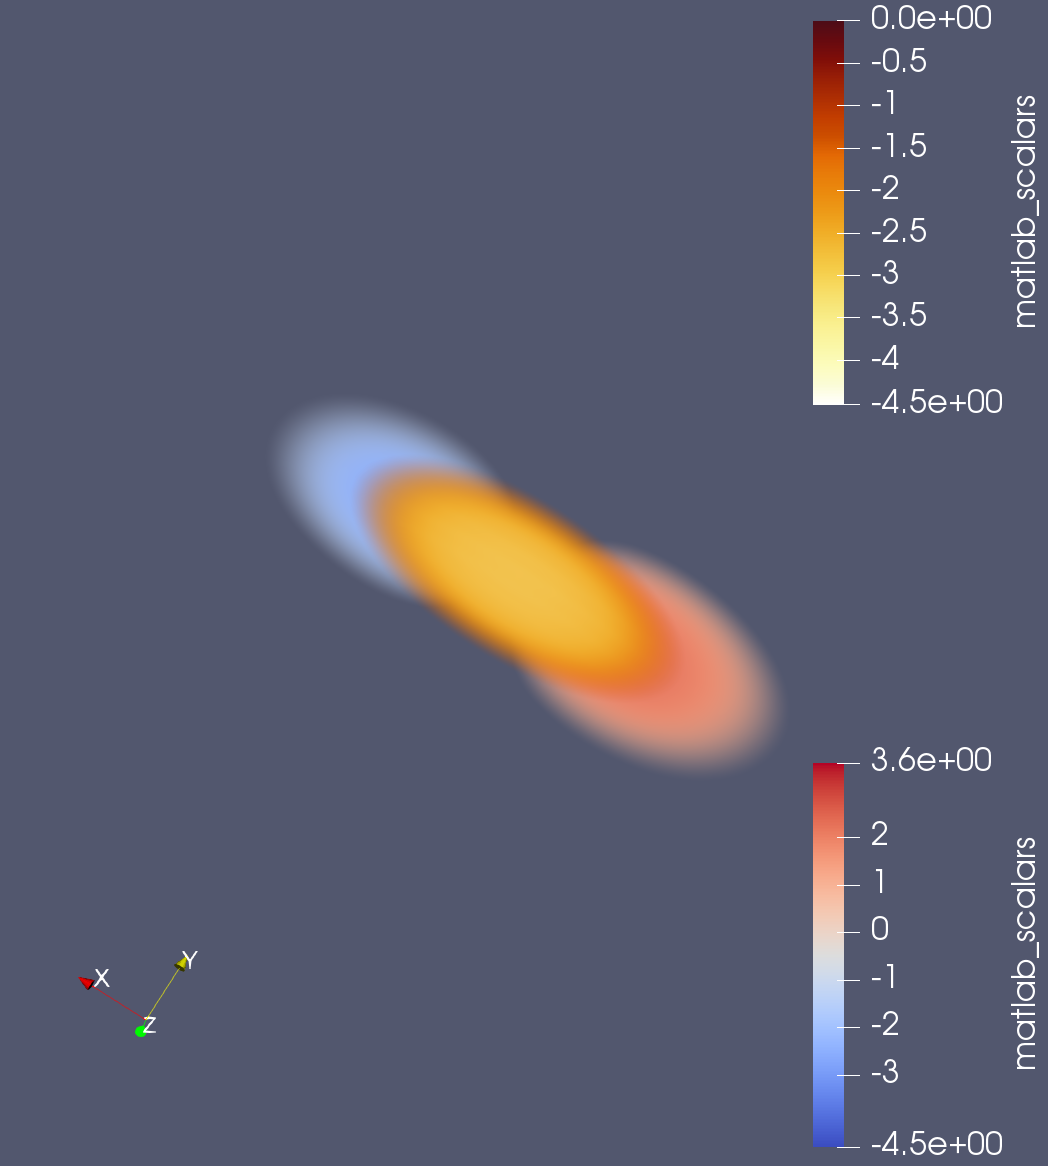
\includegraphics[width=0.25\textwidth]{ekets07.png}}
	\hspace{1em}
	\subfigure[$\ket{0}$, $\ket{8}$.]{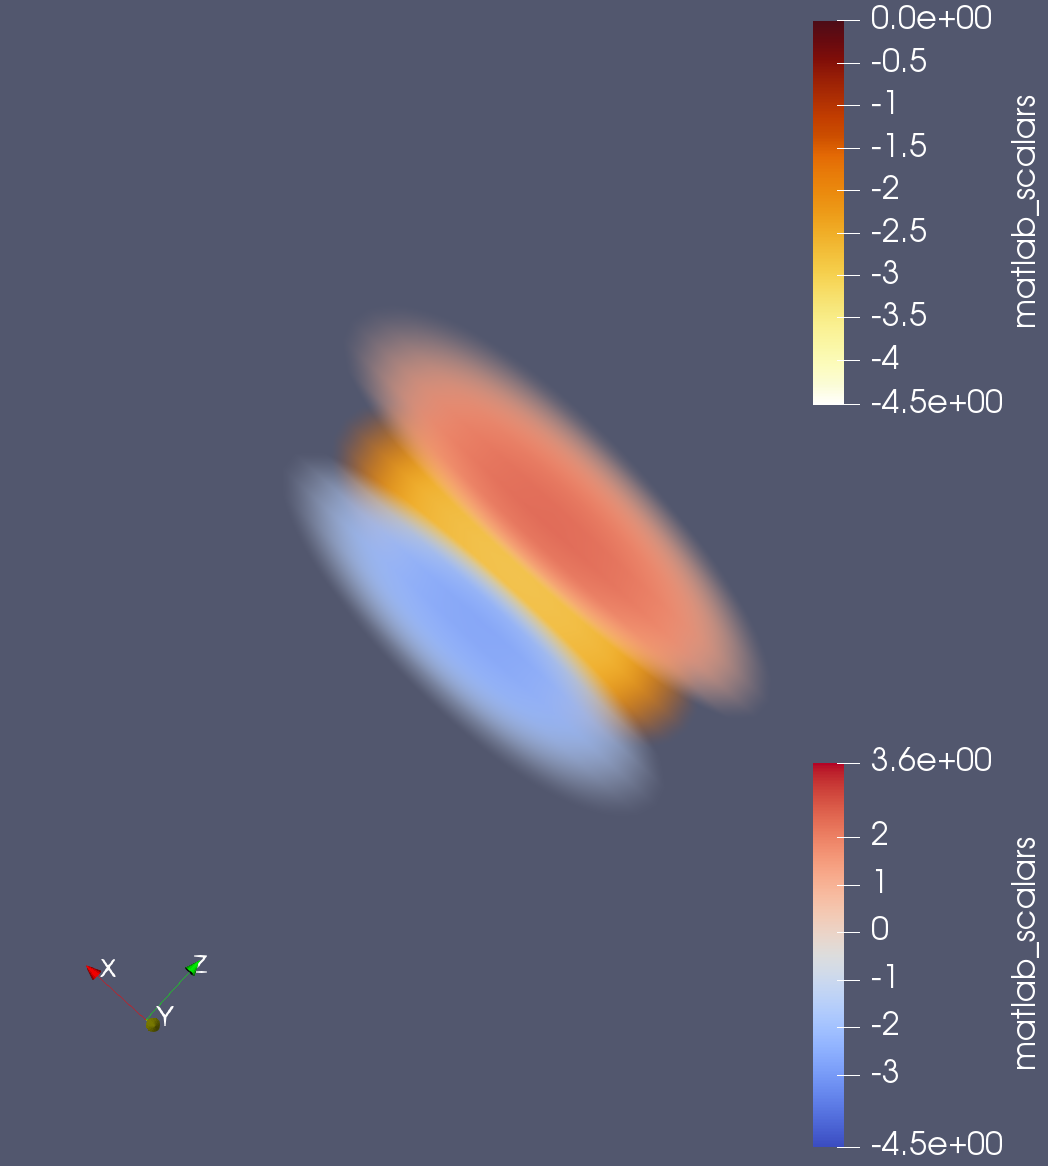
\includegraphics[width=0.25\textwidth]{ekets08.png}}
	\hspace{1em}
	\subfigure[$\ket{0}$, $\ket{9}$.]{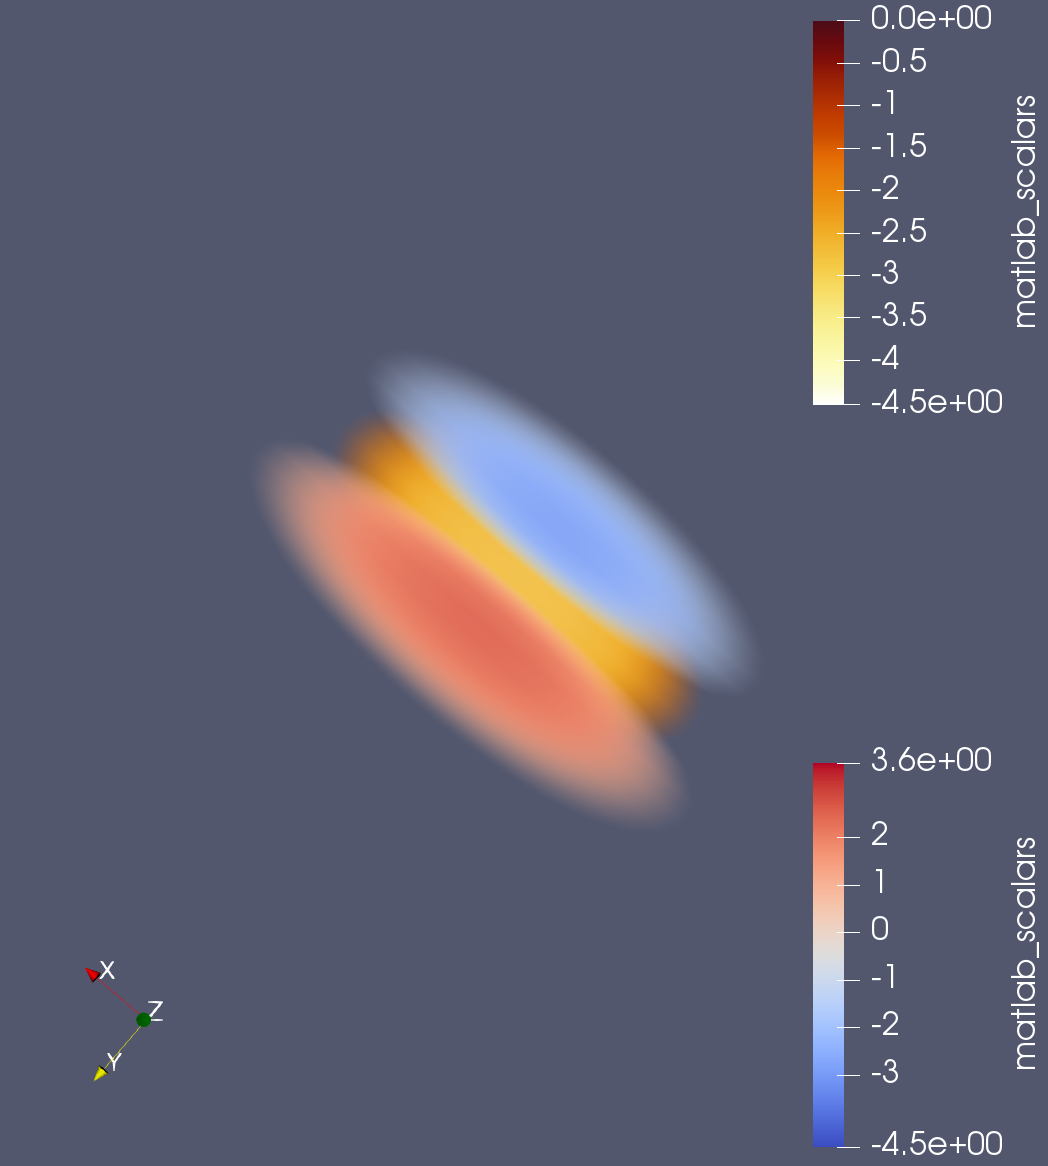
\includegraphics[width=0.25\textwidth]{ekets09.png}}
\end{figure}
\end{frame}




\begin{frame}[shrink=10]
\frametitle{Capacitative coupling}
\vspace{2em}
TDPT: for perturbation $U(\vec{r}) \cos{\omega t}$
\begin{equation}
P_{i \rightarrow j} \approx \frac{\abs{U_{ij}}^2}{\hbar^2} \frac{\sin^2{(\omega_0-\omega)t/2}}{(\omega_0-\omega)^2}
\end{equation}
Transition matrix element depends on coupling configuration. 
\begin{minipage}[c]{0.45\linewidth}
\begin{figure}
	\centering
	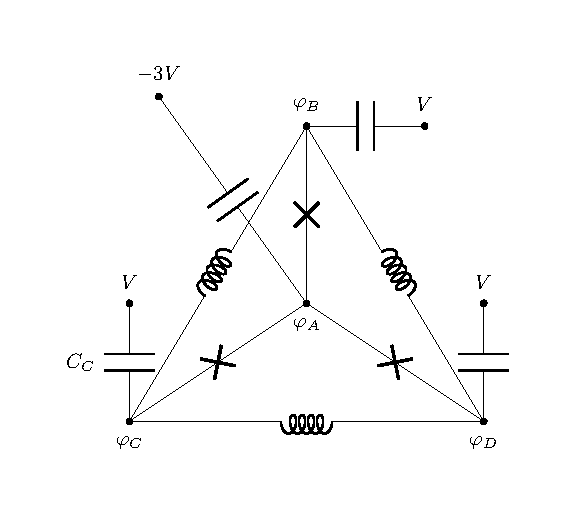
\includegraphics[trim={0cm 1cm 0cm 1cm}, clip, width=1\textwidth]{triflux_zeta_couple.pdf}
\end{figure}
\end{minipage} 
\begin{minipage}[c]{0.45\linewidth}
e.g. $\zeta$ mode
\begin{equation}
\ham = \ham_0 + 2 \sqrt{3} (2e) \frac{C_C}{C_\zeta} V \partial_\zeta
\end{equation}
\end{minipage}
\end{frame}

% exciting an atom: coupling between $\vec{E}$ field and `dipole'  



\begin{frame}
\frametitle{Capacitative coupling}
\begin{figure}
	\centering
	\subfigure{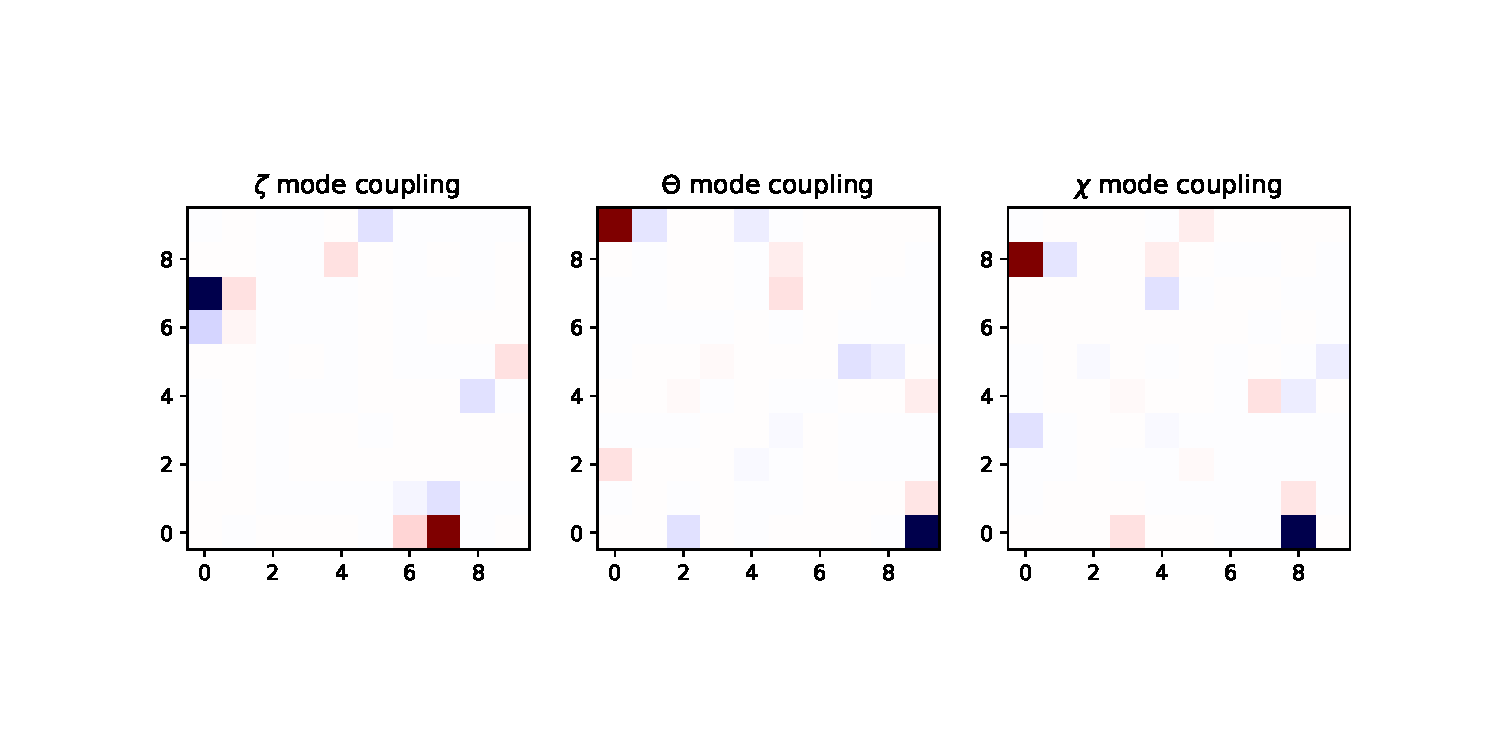
\includegraphics[trim={2cm 2.5cm 2cm 2.5cm}, clip, width=0.8\textwidth]{coupling.pdf}}
	\subfigure{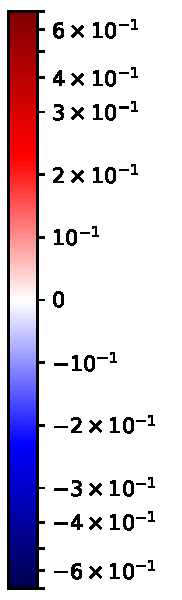
\includegraphics[trim={0cm -1cm 0cm 0cm}, clip, width=0.07\textwidth]{coupling_colorbar.pdf}}
\end{figure}

Possible scheme: $\ket{0}$, $\ket{1}$ for logical 0, 1 respectively. $\ket{7}$ as the intermediate state for a multistep transition.
\end{frame}

% though experimentally, large energy gap between 0 and 7 is difficult


\end{document}